\section{Lezione 2016-11-07}
\subsection{TODO}
% Insert what you need. Any row is associated with the improvment or mistake
% arise. In the first column you can insert what you should resolve or change,
% instead in the second column you may put the section where to apply some
% modification.
\begin{table}[H]
\begin{center}
\begin{tabular}{|p{\textwidth}|c|}
\hline
\multicolumn{1}{|c|}{\textbf{Miglioramento}} & \textbf{Sezione} \\ \hline
Chiarire la dicitura \textbf{OK} nell'algoritmo $getReg$ &
\ref{alg:gerReg} \\ \hline
\end{tabular}
\end{center}
\caption{Tabella miglioramenti}
\label{tab:tab_todo}
\end{table}

\subsection{Generatore di codice}
\begin{definition}[Code generator]
Un generatore di codice \`e un algoritmo per generare codice target per un
blocco base (sequenze di istruzioni \textit{three-address code}) usando la
\textit{next-use information} (locale).
\end{definition}

Il problema maggiore \`e l'utilizzo dei \textbf{registri}. Vi sono varie
tecniche affinch\`e i registri vengano sfruttati con efficenza.

\subsubsection{Next-Use Information (locale)}
La \textit{next-use information} \`e necessaria l'\textbf{eliminatione} del
codice morto e l'\textbf{assegnazione} dei registri. La \textit{next-use} \`e
calcolata mediante scansione all'indietro (\textit{backward}) di un blocco base
ed esegue le seguenti azioni su istruzioni $L: \ x := y \ op \ z$:
\begin{enumerate}
\item Aggiunge un' informazione \textit{next-use/viva} su $x,y$ e $z$
all'istruzione $L$ (informazione archiviata nella tabella dei simboli)
\item Salendo alle istruzioni precedenti (\textit{scan up}):
\begin{itemize}
\item informazioni di $x$: \textit{not live} e \textit{no next use}
\item informazioni di $y,z$: \textit{live} e \textit{next use}$\ =L$
\end{itemize}
\end{enumerate}

Al primo passo, l'ultima istruzione, tutte le variabile sono \textbf{vive}
senza nessun uso successivo (etichetta istruzione dove verr\'a riutilizzata).
Queste informazioni vengono assegnare all'ultima informazione di cui in seguito
si calcola la sua \textit{next-use information}, come in
fig.\ref{img:next-use}. L'informazione calcola sar\'a attaccata all'istruzione
precedente. Il processo continua fich\`e ogni informazione ha il suo
\textit{next-use information} (fig.\ref{img:second_step_next-use}).

\begin{figure}[H]
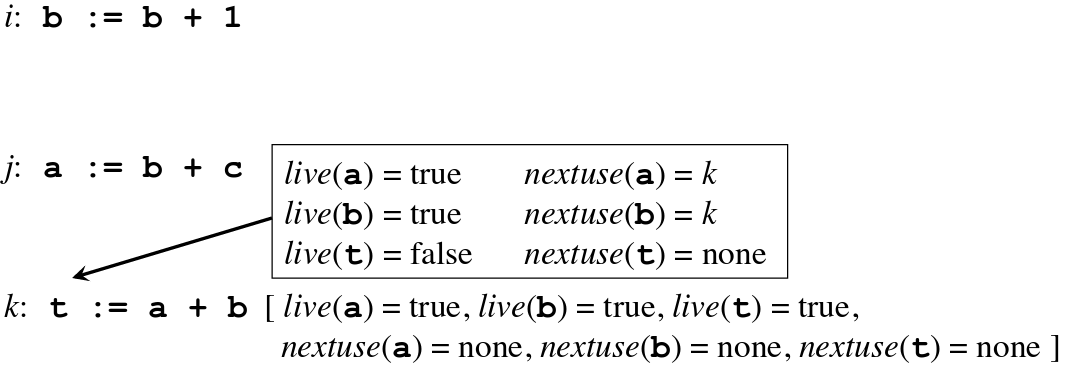
\includegraphics[scale=0.4]{res/image/next-use}
\caption{Primo passaggio per calcolo del \textit{next-use}}
\label{img:next-use}
\end{figure}

\begin{figure}[H]
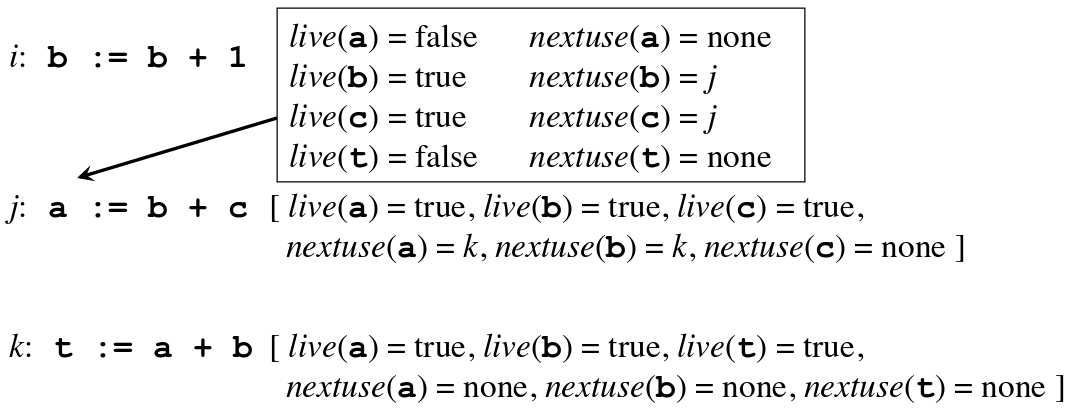
\includegraphics[scale=0.4]{res/image/second_step_next-use}
\caption{Passaggio successivo per calcolo del \textit{next-use}}
\label{img:second_step_next-use}
\end{figure}

\subsection{Abbozza del generatore}
Per ogni istruzione \textit{three-address code} l'algoritmo esegue le
operazioni in modo da conseguire i comandi avendo tutte le risorse (operandi)
nei registri:
\begin{enumerate}
\item Controllo assenza operandi nei registri, invio \textbf{loads}
corrispondente
\item invio operazioni
\item invio \textbf{store} del risultato, se necessario
\end{enumerate}

L'algoritmo fa uso dell'\textit{address descriptors}, del
\textit{register descriptors} ed una funzione $getReg$ il quale
$getReg=(x=y \ OP \ z)$ ritorna i tre registri da utilizzare per $x,y,z$
(denotati come \textit{Rx,Ry} e \textit{Rz}).

\subsubsection{Descrittore indirizzi e registri}
I descrittori servono per mantenere la posizione delle risorse
(indirizzi, variabili) necessarie all'esecuzione del programma.

\paragraph{Register descriptor (RD)}
tiene traccia delle variabili di cui il valore corrente nel registro.
\paragraph{Address descriptor (AD)}
tiene traccia del luogo dove il valore corrente della variabile potr\`a
essere trovato.

L'RD lavora per ogni registro disponibile, invece l'AD per ogni variabile.

Con \textbf{luogo} si pu\'o intendere un registro ma anche posizioni nello
stack, indirizzi di memoria e cosi via. Quest'informazione potr\'a essere
salvata nella tabella dei simboli.

\subsubsection{Algoritmo del generatore}
\paragraph{Per istruzioni \textit{three-address code} ($x = y \ OP \ z$)}
\begin{itemize}
\item usa $getReg=(x=y \ OP \ z)$ per selezionare i registri \textit{Rx,Ry} e
\textit{Rz} per $x,y,z$.
\item se $y$ non \`e in \textit{Ry}, si invia un'istruzione \textit{LD Ry,$y'$}
dove $y' \in AD(y)$, preferibilmente un registro
\item similarmente per $z$
\item invia l'istruzione \textit{OP Rx,Ry,Rz}
\end{itemize}

\paragraph{Istruzioni di copia ($x=y$)}
\begin{itemize}
\item se $y$ non \`e gi\'a nel registro, invia \textit{LD Ry,$y'$}
\item regola $RD$ per \textit{Ry} cosi da includere $x$
\item cambia $AD$ per $x$ cosi la sua unica posizione \`e in \textit{Ry}
\end{itemize}

\paragraph{Fine del blocco base}
\begin{itemize}
\item se $x$ \`e usato in altri blocchi, invia \textit{ST x,Rx}
\end{itemize}

\begin{algorithm}[H]
\caption{$getReg=(x:=y \ OP \ z)$}
\label{alg:gerReg}
\begin{algorithmic}
\Function {getRegisterFor}{$a$}
\If {$a.isStored()$}
  \Return {$a.register()$}
\ElsIf {$isREmpty()$}
  \Return {$REmpty()$} \Comment registro come $Ra$
\Else
  \State declare $R_{min}$ \Comment R con il minimo di spill
  \State $R_{min}.spill \leftarrow \infty$
  \ForAll {$R \in getRegisters()$}
    \State $R.spill \leftarrow 0$
    \ForAll {$v \in RD(R)$}
      \If {$AD(v)-\{R\} \neq \emptyset$}
        break
      \ElsIf {$v=x$ \&\& !$live(x)$}
        break
      \ElsIf {$nextUse(v) \neq nextIstruction()$}
        break
      \Else
        \State $print(\mathbf{ST \ v,R})$
        \State $R.spill \leftarrow R.spill + 1$
      \EndIf
    \EndFor
    \State $R_{min} \leftarrow \underset{spill}{min}(R_{min},R)$
  \EndFor
  \State \Return $R_{min}$
\EndIf
\EndFunction
\\
\Function {getRegisterForX} {$Ry,Rz$}
\If {$noMoreUsed(y) \ \&\& \ RD(Ry)=\{y\}$}
  \State \Return $Ry$
\ElsIf {$noMoreUsed(z) \  \&\& \ RD(Rz)=\{z\}$}
  \State \Return $Rz$
\Else
  \State \Return $getRegisterFor(x)$
\EndIf
\EndFunction
\\
\State declare $Ry \leftarrow getRegisterFor(y)$
\State declare $Rz \leftarrow getRegisterFor(z)$
\State declare $Rx \leftarrow getRegisterForX(Ry,Rz)$
\end{algorithmic}
\end{algorithm}

\begin{algorithm}[H]
\caption{$getReg(x:=y)$}
\label{alg:getRegEq}
\begin{algorithmic}
\State declare $Ry \leftarrow getRegisterFor(y)$
\State declare $Rx \leftarrow Ry$
\end{algorithmic}
\end{algorithm}

Il generatore basato sull'algoritmo $getReg$ non \`e ottimale; tutte le
variabili vive nei registri sono archiviate alla fine di un blocco:
\textbf{questo potrebbe non essere necessario}.

Il \textbf{registro globale di allocazione} assegna le variabili ad un numero
limitato di registri e attende di tenere questi registri consistenti tra i
confini dei blocchi base.

Gruppi di registri possono essere dedicati a certi valori (indirizzi base,
aritmetici, puntatori allo stack). Ci\'o semplifica il generatore ma di contro
vi \`e un uso meno efficiente dei registri.

\subsubsection{Allocazione registri nel loop}
Supponiamo i seguenti benefici:
\begin{itemize}
\item non immagazzianare una variabile $x$ ha un beneficio di 2
\item accedere alla variabile invece che alla memoria ha un beneficio di 1
\end{itemize}

inoltre dichiriamo:
\begin{itemize}
\item $use(x,B)=$ numero di uso $x$ in $B$ prima dell'assegnamento
\item $live(x,B)=1$ se $x$ \`e assegnata in $B$ e vive all'uscita da $B$
\end{itemize}

\begin{definition}[Benefit]
Il beneficio (approssimato) d'allocazione di una variabile $x$ in un registro
all'interno di un loop $L$ \`e
$$\sum_{B \in L}(use(x,B)+2live(x,B))$$
\end{definition}

\subsection{Allocazione dei registri globali con il grafo dei colori}
Quando un registro \`e necessario ma tutti i registri avviabili sono in uso,
il contenuto di uno dei registri usati deve essere archiviato
(\textit{spilled}) per liberare il registro.

Attraverso un grafo dei colori si va ad allocare i registri e tenta di
minimizzare il costo degli \textit{spill}. Primo bisogna costruire il grafo dei
\textbf{conflitti} (o grafo d'interferenza): abbiamo un nodo per ogni variabile
viva e due variabili hanno un vertice se una \`e viva dove l'altra \`e
definita. Infine bisogna trovare il grafo a k-colori dove i colori sono i
registri.

\begin{figure}[H]
  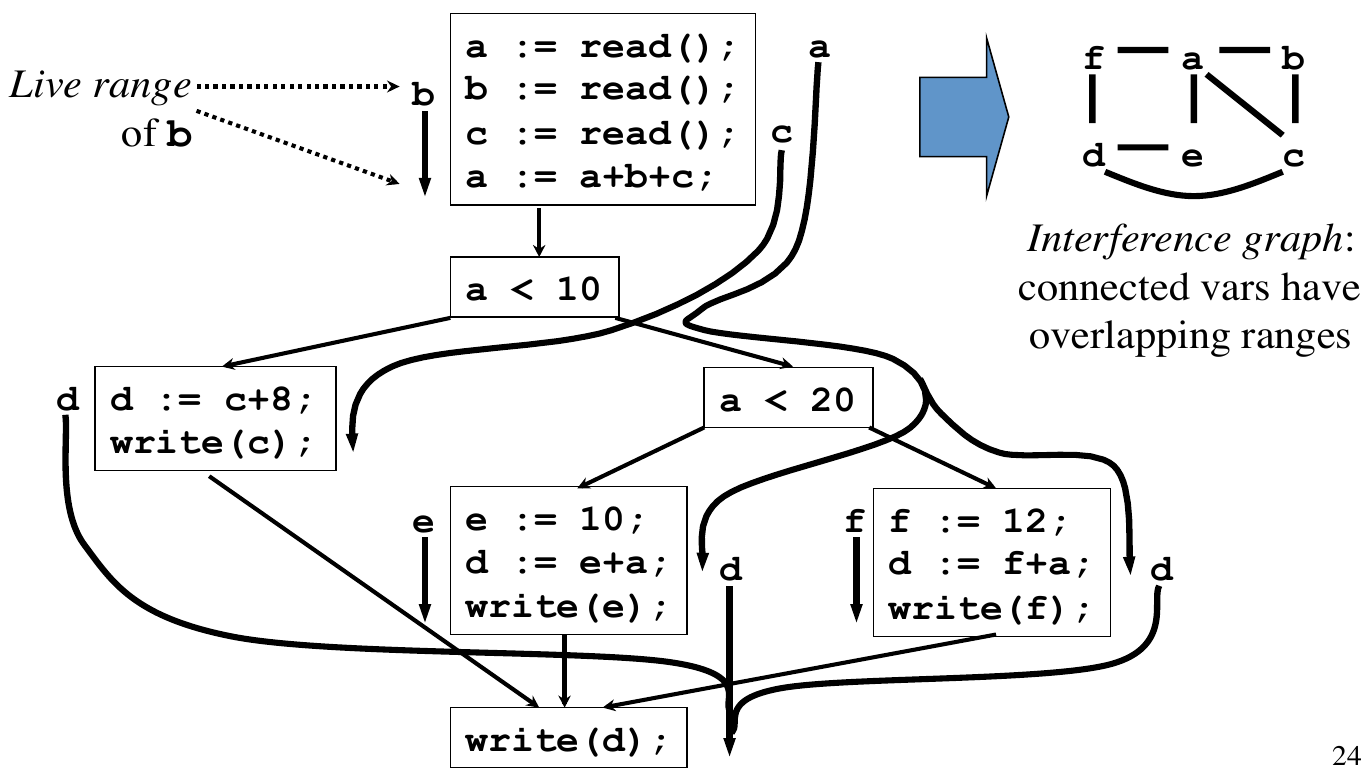
\includegraphics[scale=0.4]{res/image/interference_graph}
  \caption{Costruzione grafo d'interferenza}
  \label{img:interference_graph}
\end{figure}
